\section{Эйлеровы циклы и цепи в графе. Теорема об эйлеровом цикле. Выяснить, существует ли в графе 
Эйлеров цикл и цепь.}

Задача о Кёнигсбергских мостах послужила началом математической теории
графов.

Изобразим расположение мостов. Задача: выйти из любой точки, пройти по
всем мостам по одному разу и вернуться обратно.

\begin{figure}[h]
    \centering
    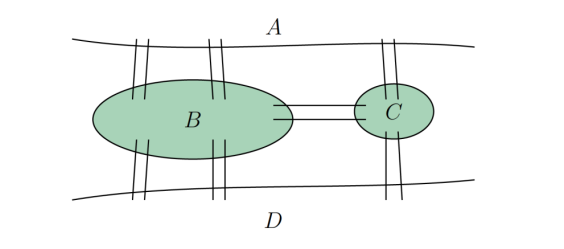
\includegraphics[scale=0.4]{20_1.png}
\end{figure}

Изобразим граф, в котором вершинами является суша, а рёбрами -- мосты.

\begin{figure}[h]
    \centering
    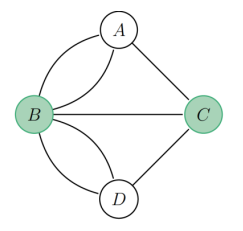
\includegraphics[scale=0.4]{20_2.png}
\end{figure}

\begin{definition}
    Если в графе есть цикл, проходящий по всем рёбрам графа, то
    такой цикл называется \textit{эйлеровым циклом}, а граф называется \textit{эйлеровым
    графом}.
\end{definition}

\begin{theorem}
    Конечный граф без изолированных вершин является эйлеровым
    графом если он является связным и степени всех его вершин четные числа.
    \begin{figure}[h]
        \centering
        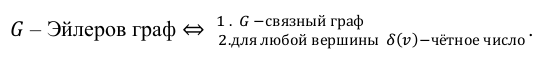
\includegraphics[scale=0.5]{20_3.png}
    \end{figure}
\end{theorem}

\begin{proof}
    $\Rightarrow$ $G$ -- эйлеров граф. По определению, в графе есть эйлеров граф.
    Значит граф связный.

    Каждый раз, проходя через вершину, цикл заходит в эту вершину по одному
    ребру, а выходит по другому ребру. То есть при прохождении через вершину
    задействуется два различных ребра. Так как в эйлеров цикл входят все рёбра
    графа, то степень каждой вершины -- четное число.

    $\Leftarrow$ Пусть граф является связным и степени всех его вершин четные числа.
    Построим в графе $G$ эйлеров цикл. Начнём цикл в произвольной вершине $a$.
    Из вершины $a$ будем строить цикл, проходя всё время по разным рёбрам. Так
    как степень каждой вершины -- чётное число, то цикл может завершиться
    только в вершине $a$.

    Обозначим полученный цикл за P. Если в $P$ входят все рёбра графа $G$, то получили
    эйлеров цикл. Пусть в $P$ входят не все рёбра графа $G$, тогда удалим из графа $G$ все рёбра,
    принадлежащие циклу $P$. Полученный граф обозначим графом $G_1$. Так как в
    графе $G$ степени всех вершин чётные, при прохождении по циклу $P$
    задействуется чётное число рёбер, инцидентных каждой вершине, то в графе $G_1$
    степень каждой вершины также чётна.
    Так как $G$ -- связный граф, то среди вершин цикла $P$ найдётся вершина $b$,
    инцидентная какому то рёбру графа $G_1$.

    Из вершины $b$ в графе $G_1$ снова строим цикл. Получим цикл, который
    завершится в точке $b$. Назовём его ${P}'$. Рассмотрим цикл, полученный
    объединением маршрутов $P(a,b), {P}', P(b,a)$. Получили цикл, содержащий
    больше рёбер, чем в первоначальном. Этот цикл возможно будет эйлеровым.
    Если нет, то процесс продолжим.
    Так как граф конечный, то этот процесс завершится на некотором шаге.
    
    В итоге получим эйлеров цикл.
\end{proof}